% !TEX program = pdflatex
% !TEX options = -shell-escape -synctex=1 -interaction=nonstopmode -file-line-error "%DOC%"

\documentclass[a4paper,11pt]{article}
\usepackage[T1]{fontenc}
\usepackage[utf8]{inputenc}
\usepackage[english]{babel}
\usepackage[bookmarks]{hyperref}
\usepackage{minted}
\usepackage{amsmath}
\usepackage[titletoc,title]{appendix}
\usepackage[ampersand]{easylist}
\usepackage{tikz}
\usepackage{pgf-umlsd}
\usepackage{microtype}
\DisableLigatures[>,<]{encoding = T1,family=tt*}
\usepgflibrary{arrows}
\usetikzlibrary{automata, positioning, arrows}

\usemintedstyle{emacs}
\hyphenation{lista double-linked}
\hyphenation{linkata}
\hyphenation{thread}
\hyphenation{ges-tione}

\begin{document}
\begin{titlepage}


\definecolor{unipi-blue}{RGB}{14, 50, 128}

\title{%
\includegraphics[width=0.3\textwidth]{Stemma_unipi.jpg}~ 
\\[1cm]
Computer Networks Lab,
\\Word Quizzle project essay.
\\UniPi, Computer Science dept.
}
\author{Tommaso Colella
\\ 545625}
\date{January 14, 2020}
\maketitle
\thispagestyle{empty}
\tableofcontents
\end{titlepage}

\newpage

\section{Design choices}
%\addcontentsline{toc}{section}{Design choices}
Hereafter are presented the design choices taken during the development of the Word Quizzle game.

\subsection{General Architecture}
I chose to implement the Word Quizzle server class using a using a mixed approach of Selectors and Threadpool. 

The Selector in the server loop was chosen in order to avoid unnecessary thread spawning. It accepts new connections and subsequently multiplexes logged clients' sockets in order to get readability status and generate tasks for the Threadpool.
Another Selector is used for multiplexing purposes inside the MatchTask. Please refer to the included javadocs for a better explanation.

The Threadpool is in charge of executing tasks generated inside the Selector loop. It has a core size of 4 Threads since most CPUs nowadays support a minimum of 4 threads. The server state changes caused by the task executions are made possible thanks to the ConcurrentHashMap instances  described in the next section.

I used the WQWords class in order to extract a specific number of words from a dictionary called \texttt{ItalianDictionary.txt} and ask for their translations (since there could possibly be more than one) to the MyMemory remote API.

The Word Quizzle client implements a simple loop waiting for user input by means of a Console class instance, subsequently sending the input to the remote server and waiting for an answer. The client side match logic is only slightly more complex than the main loop, please refer to the included javadocs for a more detailed explanation. A dedicated Thread is run by the client in order to wait for incoming Datagrams bringing match requests with them.

The open source GSON library, mainly developed by Google, has been used for serialization and deserialization purposes.

\subsection{Data structures}
Throughout the whole project the  \texttt{ConcurrentHashMap} data structure was heavily used. This choice was made in order to support concurrent retrievals of various kinds of data, including online IPs, usernames and WQUser instances.

The core class \texttt{WQDatabase} uses a ConcurrentHashMap to store WQUser instances, including users' nicknames and scores.

Inside WQWords we used an ArrayList<String> to store the dictionary line by line and an HashMap<String, ArrayList<String>{}> to return the word-translations mapping to the WQServer.

The ConcurrentHashMap (and the simple HashMap as well) class permits fast O(1) retrievals provided we have a key to look up.


\subsection{Activated Threads}
The client only activates a single Thread (apart from the main one). The UDPListener thread, as previously specified, is used for the purpose of waiting for user challenges.

The server only runs a single thread to multiplex i/o and has a Threadpool with a core size of 4 and a potentially unlimited maximum pool size (bounded only by the MAXINT value) for task completion purposes. This permits an arbitrary number of threads to be spawned in case of heavy load, but these threads despawn after 100 milliseconds of idle time as per the used ThreadPoolExecutor constructor.

\subsection{Concurrency control}
The only place in which a real concurrency control takes place is inside the WQDatabase class. Some of the methods are declared as synchronized to avoid race conditions with WQUser instances insertions and to ensure a correct serialization.

\smallskip

\section{Classes}
%\addcontentsline{toc}{section}{Classes}
%\renewcommand*{\theHsection}{chY.\the\value{section}}
%\setcounter{section}{1}
Hereafter the Word Quizzle classes are neatly presented. For an in depth description and for execution methods please refer to the javadocs (where the constructor parameters are thoroughly described) and to the commented code.
\begin{itemize}
    \item \texttt{WQServer.java}
    
    Its purpose is to set up everything in order to serve client requests and to build the correct tasks. To do so it employs various data structures, a Selector for non blocking IO supporting multiple clients and a Threadpool. 
    
    \item \texttt{WQClient.java}
    
    The WQClient class is a simple request-response blocking client. It connects to the server specified by a command line hostname and is then used to access Word Quizzle's server functionalities. It also calls a remote method on the server for user registration purposes and has a dedicated thread to wait for user challenges.

    \item \texttt{WQWords.java}
    
    This class was created to extract words from the dictionary and to get their translations from the MyMemory API.
    
    \item \texttt{WQDatabase.java}
    
    The WQDatabase class acts as a buffer between the filesystem and the WQServer. It implements methods to serialize and deserialize the Database.json and provides getter and setter methods to access for its inner data.
    There's only a single instance of it, so it works like a Singleton (even though I didn't code any mean to avoid more instances to be instantiated)
    
     \item \texttt{WQUser.java}
     
     The WQUser class models the user of the Word Quizzle game. It has the user's attibutes and a compareTo method used for scoreboard sorting purposes.
     
     \item \texttt{WQRegistrationRMI.java}
     
     Remote Interface for the user registration RMI. The actual implementation of the class is inside the WQServer, which is the exported remote object.
     
     \item \texttt{*Task.java}
     
     The *Task classes model the logic behind each client request. For an in depth description of these classes please refer to the javadocs. 
    
    \end{itemize}



\newpage
\begin{appendices}

\section{How to compile and execute}
\subsection{Compile instructions}
Just use 
\\ \texttt{javac -cp ./:lib/gson-2.8.6.jar WQServer.java}
\\ \texttt{javac -cp ./:lib/gson-2.8.6.jar WQClient.java}
\\ in order to compile the classes to Java bytecode.

\subsection{Execution instructions}
To run Word Quizzle locally use:
\\ \texttt{java -cp ./:lib/gson-2.8.6.jar WQServer}
\\ \texttt{java -cp ./:lib/gson-2.8.6.jar WQClient localhost}

Always include an argument to WQClient's execution: either the server's hostname or "\texttt{--help}" if you want an explanation on the different client commands available 

\section{Cool and pretty useless graphs}
\subsection{Client Finite State Automaton}
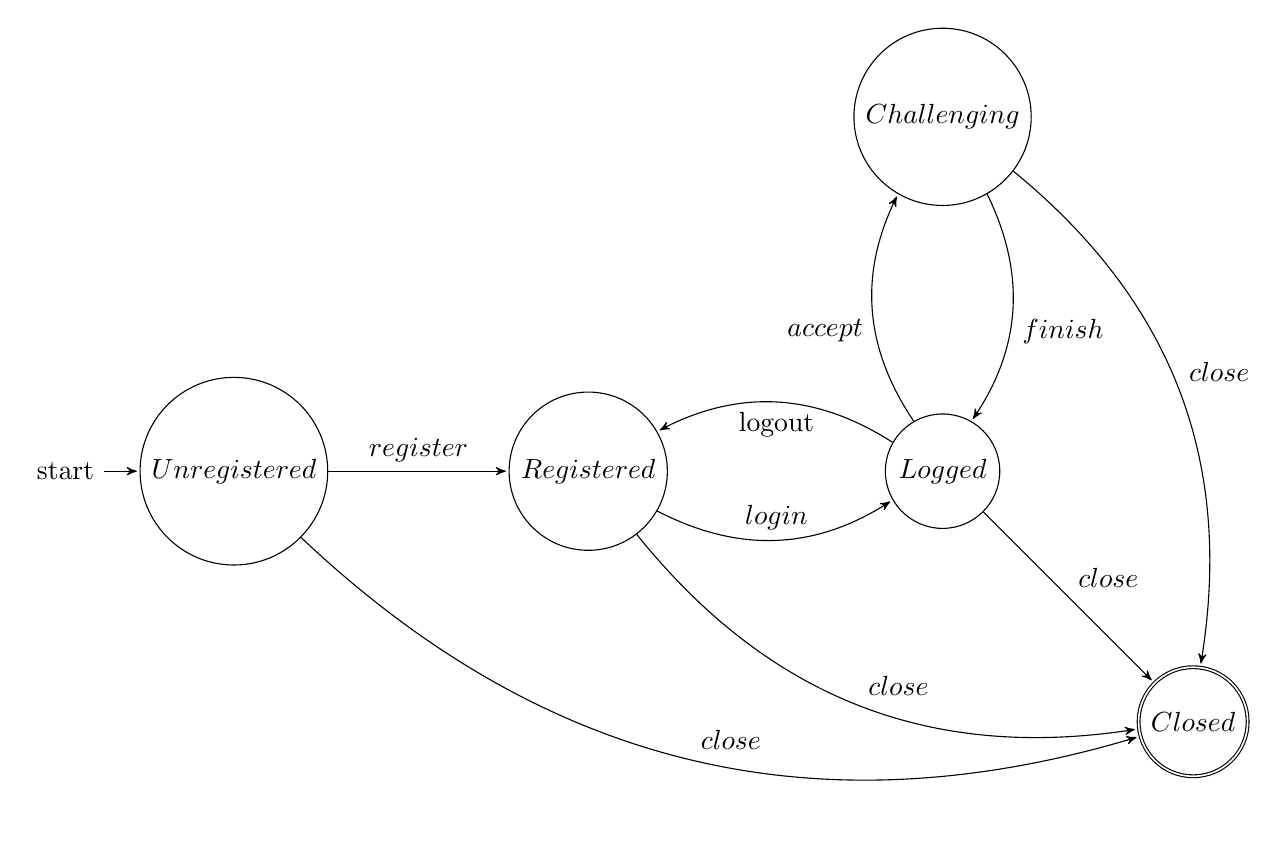
\begin{tikzpicture}[->,>=stealth',shorten >=1pt,auto,node distance=4.5cm,
        scale = 1,transform shape]

  \node[state,initial] (Unregistered) {$Unregistered$};
  \node[state] (Registered) [right of=Unregistered] {$Registered$};
  \node[state] (Logged) [right of=Registered] {$Logged$};
  \node[state] (Challenging) [above of=Logged] {$Challenging$};
  \node[state,accepting] (Closed) [below right of=Logged] {$Closed$};

  \path (Unregistered) edge             node {$register$} (Registered)
        (Registered) edge     [bend right]         node {$login$} (Logged)
        (Logged) edge         [bend left]     node {$accept$} (Challenging)
        (Logged) edge         [bend right]     node {logout} (Registered)
        (Challenging) edge          [bend left]    node {$finish$} (Logged)
        (Registered) edge     [bend right]         node {$close$} (Closed)
        (Unregistered) edge  [bend right]            node {$close$} (Closed)
        (Logged) edge              node {$close$} (Closed)
        (Challenging) edge     [bend left]         node {$close$} (Closed);

\end{tikzpicture}

\subsection{Match UML Sequence Diagram}

Below you can see simplified (and ugly) UML Sequence Diagram (Figure 1) modeling the match sequence from the viewpoint of the match sender. The slanted arrows represent UDP messages.
\newline
\newline

\begin{figure*}[!h]
    \centering
    \begin{sequencediagram}
    \begin {sdblock}[green!20]{Match Loop}{}
        \tikzstyle {inststyle}+=[top color = blue]
        \newthread{c}{:Client}
        \tikzstyle {inststyle}+=[top color = yellow]
        \newthread{s}{:Server}
        \tikzstyle {inststyle}+=[top color = green]
        \newthread{t}{TPoolThread}
        \tikzstyle {inststyle}+=[top color = red]
        \newthread{f}{:Friend}
        \mess{c}{match}{s}
        \begin{callself}{s}{new MatchTask()}{}
        \end{callself}
        \mess{s}{submitTask}{t}
        \begin{callself}{t}{run()}{}
        \end{callself}
        \mess[1]{t}{matchRequest}{f}
        \mess[1]{f}{acceptMatch}{t}
        \mess{t}{communicateAcceptance}{c}
        \mess{c}{start}{t}
        \mess{t}{firstWord}{c}
        \mess{c}{translation}{t}
        \mess{t}{lastWord}{c}
        \mess{c}{lastTranslation}{t}
        \begin{callself}{t}{calculateResults()}{}
        \end{callself}
        \mess{t}{communicateResults}{c}
    \end{sdblock}
    \end{sequencediagram}
    \caption{
This UML diagram represents the match sequence from the client's viewpoint.
}
\end{figure*}

\newpage

\section{Some self criticism}
I know I could've used a Factory design pattern in order to avoid writing unnecessary boilerplate code in each *Task method, I regret not doing so early in development.

Another cool improvement would making WQDatabase a real Singleton, but I felt it would be overkill to actually change the code at this deveopment stage for a non-critic application as Word Quizzle actually is. Also, this wouldn't add anything to the program's semantics.

The client could as well be designed to use non blocking input but if felt unnecessary to me since it would make interaction more complex without a real reason.

\end{appendices}    

\end{document}
